% !TEX root = tesis.tex

\chapter{Detección de partículas energéticas\\ solares en el \emph{SciCRT}}
\chaptermark{Detección de partículas}
\label{chap:cuatro}
\section{Desempeño del \emph{SciCRT} como detector de RC}

Estudios sobre el desempeño del SciCRT como detector de rayos cósmicos se encuentran en \cite{ynagai14,ysasai14}, sin embargo hacen la evaluación durante un periodo de tiempo corto y condiciones operacionales distintas a las actuales. En la presente sección enfocaré mis esfuerzos en determinar el desempeño del detector bajo las condiciones actuales de operación, con vistas a determinar su confiabilidad durante un evento de partículas solares y estimar los errores sistemáticos.

Con el fin de alcanzar este objetivo utilicé un código de simulación que incluye las descripción completa del telescopio, el cual fue desarrollado por mi colega Rocío García. Los detalles de esta simulación se presentan en \cite{garcia20}. Algunos puntos que fueron necesarios adaptar para realizar mi análisis son los siguientes:

\begin{itemize}
  \item Considerar seis tipos de partículas diferentes: neutrones, protones, $\mu^{\pm}$, $e^{\pm}$ y rayos $\gamma$.
  \item Utilizar el modelo PARMA con generador de eventos para las distribuciones de energía y de ángulos cenitales.
  \item Los parámetros de entra del modelo son los correspondientes a la localidad de Sierra Negra y el periodo de observación de Septiembre de \num{2017}.
  \item Todas los espectros de energía de las partículas usadas en la simulación se definen en un rango de \SI{10}{\mega\electronvolt} a \SI{1}{\tera\electronvolt}.
  \item Los propiedades ópticas de los materiales del detector están deshabilitadas para reducir el tiempo de computo.
  \item Se simulan en total \num{3e7} de eventos, los cuales son lanzados al detector desde una esfera de \SI{5}{\metre} de radio.
\end{itemize}

La figura \ref{fig:sim-setup} muestra la geometría usada en la simulación para inyectar las partículas al detector.

\begin{figure}
        \centering
        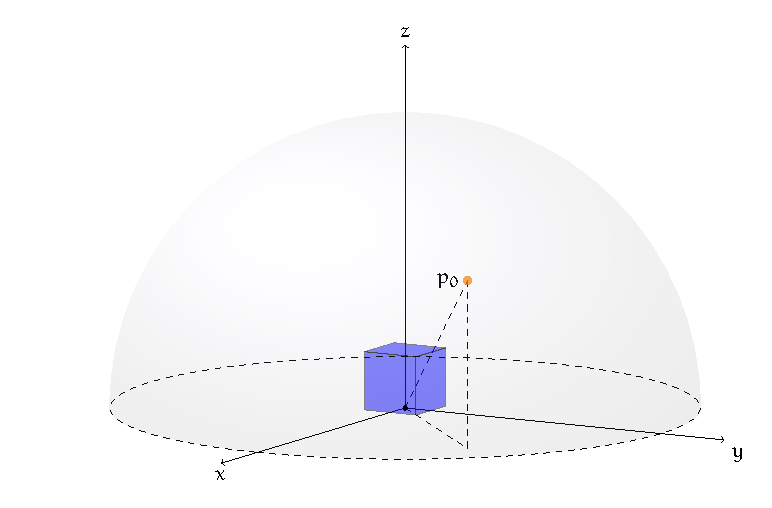
\includegraphics[width=0.75\textwidth]{sim-setup.pdf}
        \caption{Configuración de la simulación en Geant4.}
        \label{fig:sim-setup}
\end{figure}

La condición para que las partículas sean contadas en la simulación es que éstas depositen al menos \SI{7}{\mega\electronvolt} en una barra de cada lado del detector; sin generar señal en las capas dedicadas a la detección de muones. A partir de aquí selecciono solo los eventos que cumplieron con el disparo en el SB \num{3}, que es donde está instalada la electrónica de alta velocidad. El resultado de este análisis se muestra en la figura \ref{fig:total-efficiency}. La línea roja representa la eficiencia de detección de neutrones; mientras que las lineas verde, café, morada, azul y naranja son eficiencias de protones, $\mu^{\pm}$, rayos $\gamma$, positrones y electrones; respectivamente. En todos los casos las eficiencias reportadas son las totales, es decir, están ponderadas con respecto a la distribución angular e incluyen un barra de error. La tasa de eventos total estimada a partir de estas especies de \SI{3132.31(9480)}{eventos  \per\minute}, de las cuales el \SI{84}{\percent} son neutrones.

Protons are effectively rejected using the muon layers, however they are capable of entering by the sides.  About \SI{12}{\percent} of the events are produced by protons. The SciCRT has a large detection efficiency for high energy/inclined muons and $\gamma$-rays, but their contribution to the total number of events is small because these events are rare.

\begin{figure}
        \centering
        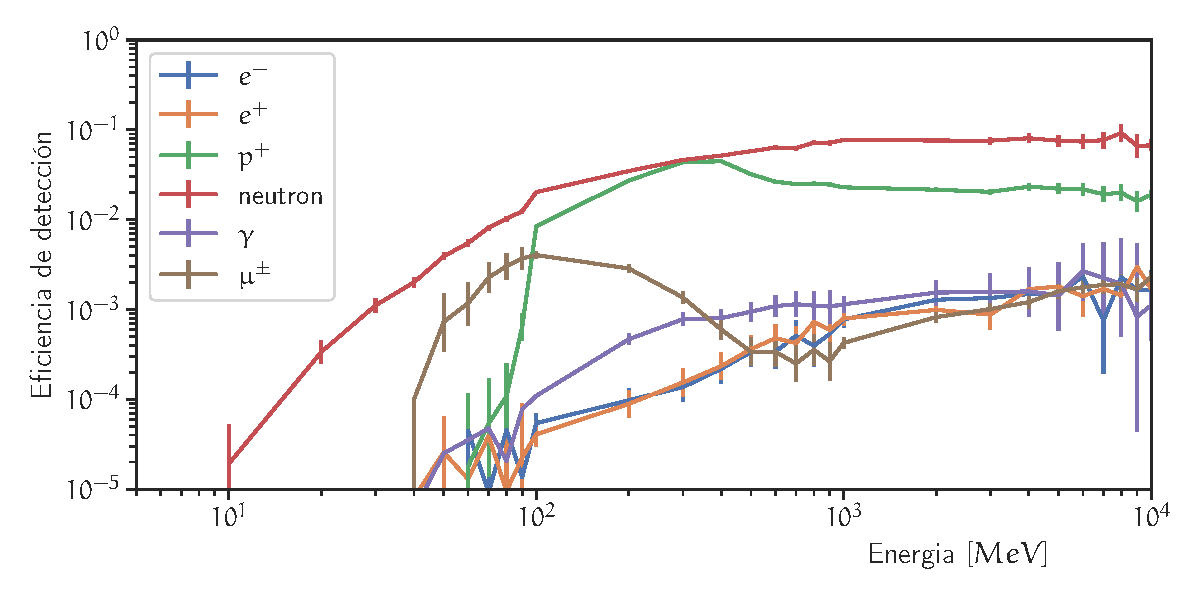
\includegraphics[width=\textwidth]{scibar-efficiency.pdf}
        \caption{Eficiencia de detección del SciCRT para diferentes especies de partículas en función de la energía incidente.}
        \label{fig:total-efficiency}
\end{figure}

\begin{figure}
        \centering
        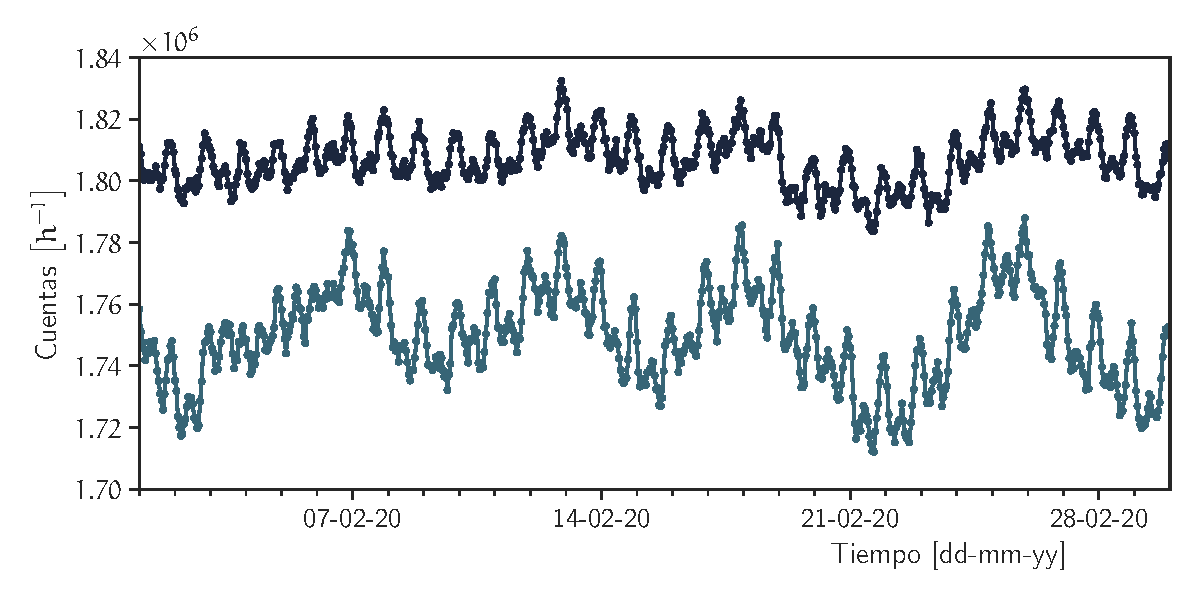
\includegraphics[width=\textwidth]{muon-monthly.pdf}
        \caption{Total de eventos de muones registrados durante Febrero \num{2020} por el SciCRT (linea azul oscura) en comparación con datos del NM de la Ciudad de México (línea azul claro).}
        \label{fig:muon-monthly}
\end{figure}

\begin{figure}
        \centering
        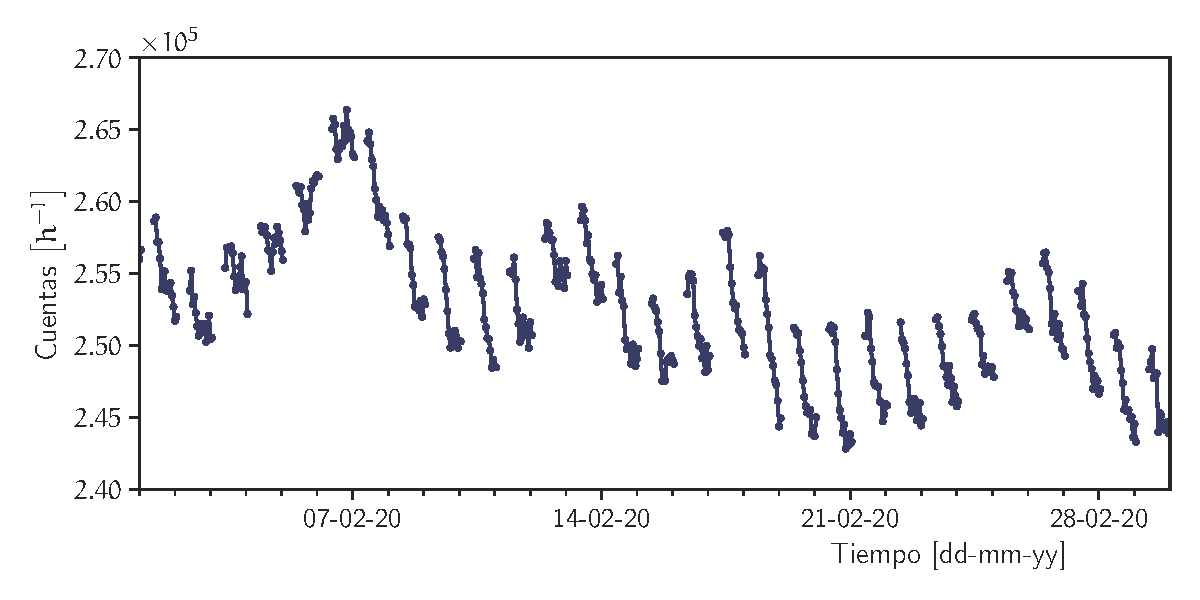
\includegraphics[width=\textwidth]{neutron-monthly.pdf}
        \caption{Total de eventos de partículas neutras registrados durante Febrero \num{2020} por el SciCRT (linea azul oscura) en comparación con datos del NM de la Ciudad de México (línea azul claro).}
        \label{fig:neutron-monthly}
\end{figure}


\begin{figure}
        \centering
        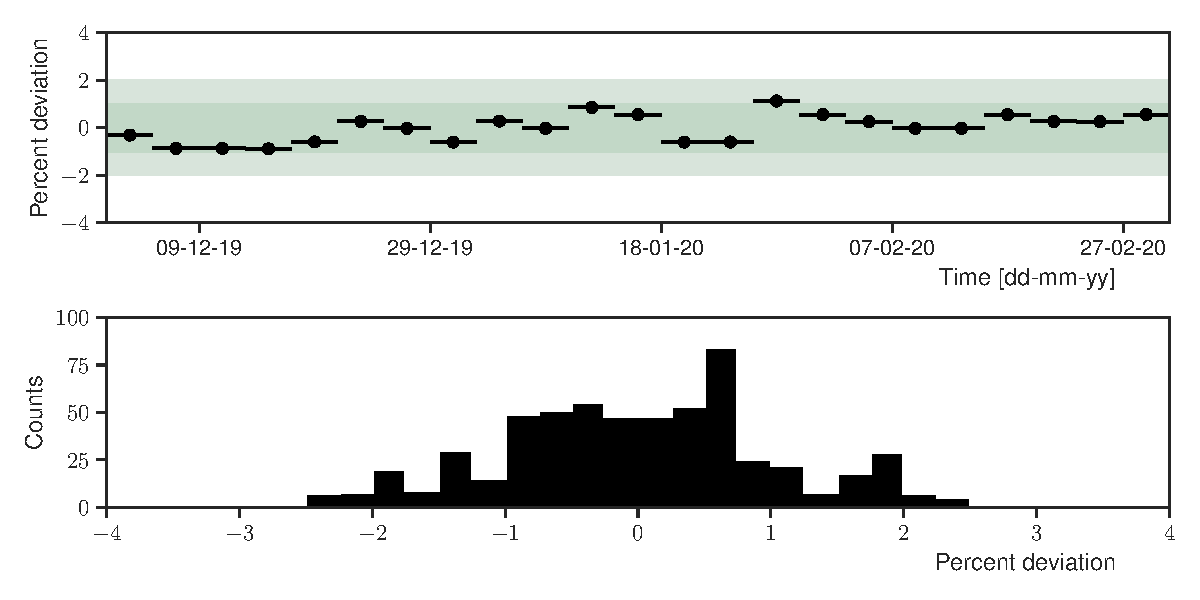
\includegraphics[width=\textwidth]{neutron-mip_stability.pdf}
        \caption{Estabilidad de la ganancia de los MAPMTs durante un periodo de tres meses. El panel superior muestra la variación en el tiempo de uno de los MAPMT. Las áreas sombreadas corresponden con las variaciones de \SI{\pm 1}{\percent} y \SI{\pm 2}{\percent}. El panel inferior es la distribución de todos los MAPMTs.}
        \label{fig:mip-stability}
\end{figure}



\begin{figure}
        \centering
        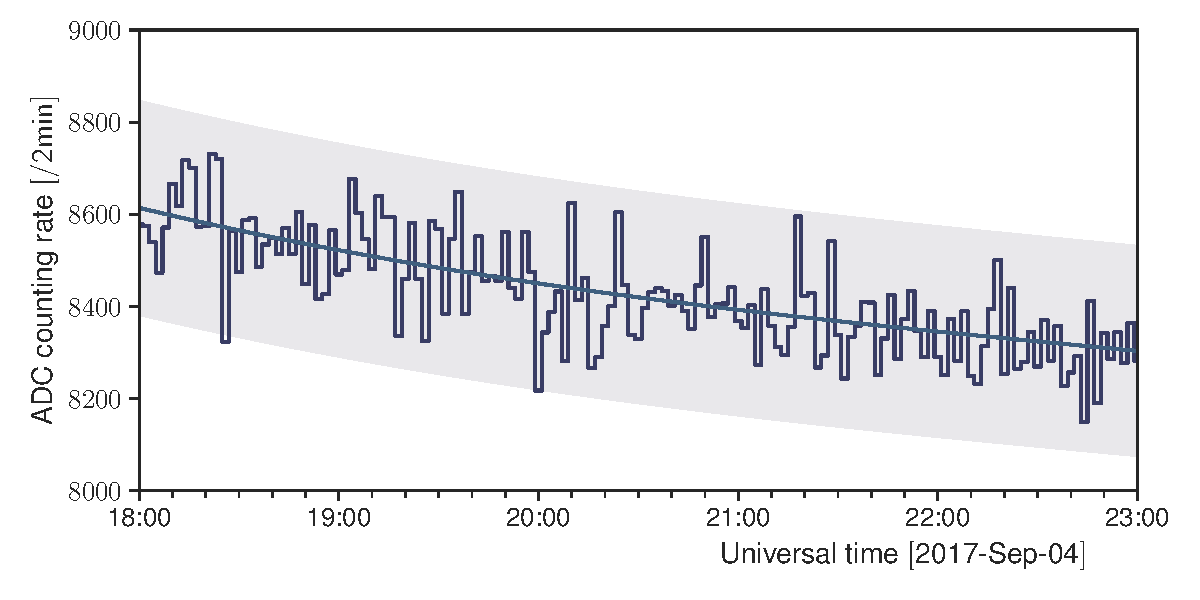
\includegraphics[width=\textwidth]{neutron-170904.pdf}
        \caption{Perfil temporal de eventos registrados por el \emph{SciCRT} el \num{4} de Septiembre de \num{2017}. El área sombreada representa el nivel de $3.0\sigma$.}
        \label{fig:september-04}
\end{figure}

\begin{figure}
        \centering
        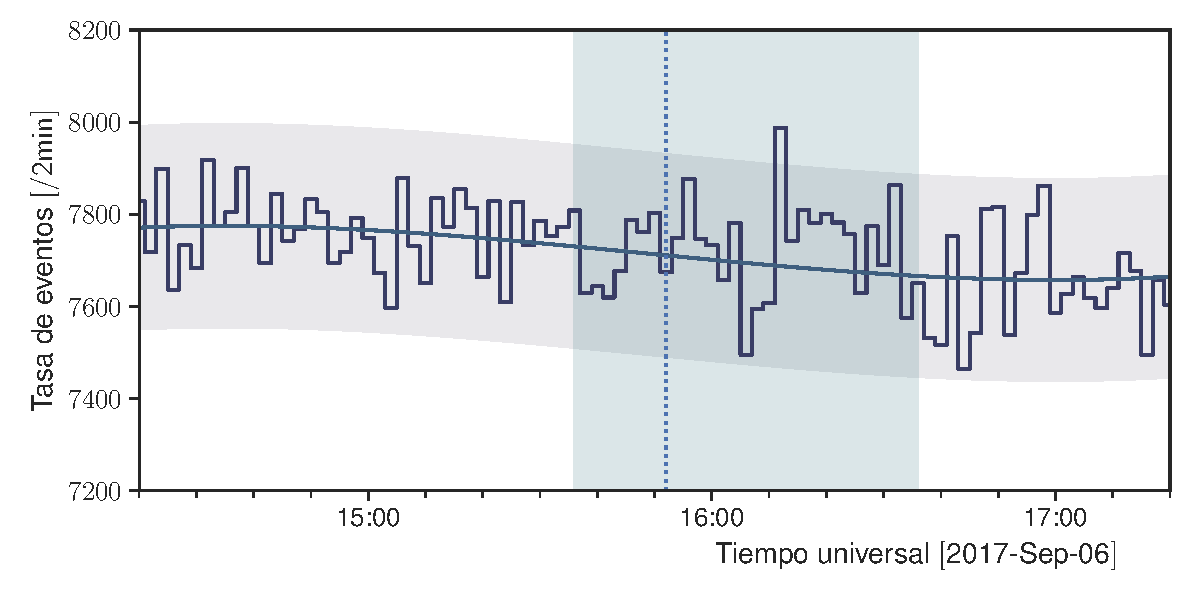
\includegraphics[width=\textwidth]{neutron-170906.pdf}
        \caption{Perfil temporal de eventos registrados por el \emph{SciCRT} el \num{4} de Septiembre de \num{2017}. El área sombreada representa el nivel de $3.0\sigma$..}
        \label{fig:september-06}
\end{figure}
